\documentclass[hyperref,envcountsame,envcountsect,runningheads]{llncs}

\usepackage[dvipsnames]{xcolor}
\usepackage{hyperref}
\pagestyle{plain}
%   \addtolength{\oddsidemargin}{-.5in}
%   \addtolength{\evensidemargin}{-.5in}
%   \addtolength{\textwidth}{1in}
\hypersetup{
    bookmarks=true,                 % show bookmarks bar?
    unicode=false,                  % non-Latin characters in Acrobat’s bookmarks
    colorlinks=true,                % false: boxed links; true: colored links
    linkcolor=RoyalPurple,          % color of internal links (change box color with linkbordercolor)
    citecolor=black,
    filecolor=black,
    urlcolor=black,
    hypertexnames=false
}
\def\topfraction{0.8}

\setcounter{tocdepth}{2}
\usepackage{domino}
\usepackage{macros}
\lstset{
  basicstyle=\tiny,
  language=Domino,
  keywordstyle=\color{kxblue}\bfseries,
  ndkeywordstyle=\color{kxpink}\bfseries,
  commentstyle=\color{gray},
}


\usepackage[math]{fontspec}
\setmonofont[Scale=MatchLowercase]{Source Code Pro}

%\usepackage[showframe,pass]{geometry}

%\makeatletter
%\let\claim\@undefined
%\let\endclaim\@undefined
%\makeatother
%\spnewtheorem{claim}[theorem]{Claim}{\bfseries}{\itshape}

% include code in verbatim
\usepackage{listings}
\lstset{
  basicstyle=\footnotesize\ttfamily,
  breaklines=true,
  numbers=none,
  tabsize=4,
  escapeinside={(*@}{@*)}
}
\usepackage{tikz}
\tikzstyle{package} = [inner sep=1pt,align=center,rounded corners,draw,minimum width=2cm,minimum height=1cm,font=\small]
\tikzstyle{onarrow} = [inner sep=1pt,font=\scriptsize,anchor=west,at start,align=left,fill=white]


\let\llncssubparagraph\subparagraph
\let\subparagraph\paragraph
\usepackage{titlesec}
%\let\subparagraph\llncssubparagraph
\let\paragraph\subsubsection
\titlespacing*{\section} {0pt}{3ex plus 1ex minus .2ex}{2.1ex plus .2ex}
\titlespacing*{\subsection} {0pt}{2.75ex plus 1ex minus .2ex}{1.3ex plus .2ex}
\titlespacing*{\subsubsection}{0pt}{1ex plus 1ex minus .2ex}{2mm}


\newcommand\defeq{\mathrel{\overset{\makebox[0pt]{\mbox{\normalfont\tiny\sffamily
def}}}{=}}}
\def\checkmark{\tikz\fill[scale=0.4](0,.35) -- (.25,0) -- (1,.7) --
  (.25,.15) -- cycle;}

% Submission version
%\newcommand{\workingnotes}[1]{}
%\newcommand{\workingnotes}[1]{\marginpar{\scriptsize{#1}}}
%\newcommand{\workingnotes}[1]{{#1}}



\todostyle{christoph}{author={\textbf{Christoph}},color=RoyalPurple!60,inline}


\title{On The Cost Of Late Binding}
%{\small ---Draft, do not distribute---}}
\author{}\institute{}
\author{Chris Brzuska\inst{1},
       Christoph Egger\inst{2},
       Amirhosein Rajabi\inst{1},
       Felix Rohrbach\inst{3},
       Gabrielius Rosinas\inst{1}}
%       Jan Winkelmann\inst{4}}
\institute{
  Aalto University, Finland \and Chalmers University of Technology and University of Gothenburg, Sweden \and CISPA Helmholtz Center for Information Security %\and Free spirit
}


% Imported from domino
%\newcommand\lit[1]{\ensuremath{\mathtt{#1}}}
\renewcommand\O[1]{\ensuremath{\mathsf{#1}}}
\newcommand{\M}[1]{\ensuremath{\text{\texttt{#1}}}}
\newcommand{\n}[1]{\ensuremath{\mathit{#1}}}




\begin{document}
\maketitle

\begin{abstract}
  In key exchange protocols, the derived key should be bound to the session. In TLS 1.3, this binding happens rather late, which has been identified as a significant source of complexity for analysing the TLS 1.3 key schedule (ASIACRYPT 2022).

We argue that the extension of TLS 1.3 would be a natural point to adapt early binding. While the computational costs of an early binding to both the ciphertext and public key of the KEM as well as the key shares of the DH would be negligible, we show the significant difference in complexity of the analysis by providing two formally verified proofs of a key exchange, once with early and once with late binding. We model the key exchange in the state separating proofs framework (SSP, ASIACRYPT 2018), and use the recently published Domino tool to verify our proofs.

\end{abstract}

\section{Introduction}
\label{section:introduction}
Since older versions of Transport Layer Security (TLS) suffered from numerous attacks~\cite{X,Y,Z}, %TODO: Heavy blanket-citing with 10 papers or so. BEAST, Lucky13...
the newest version of TLS is based on principled design and close collaboration between industry and academia.
In particular, drafts of TLS 1.3 have been extensively analyzed~\cite{X,Y,Z} %TODO: Heavy blanket-citing with 10 papers or so. Cite Cas Cremers, Marc Fischlin, Felix Günther and others.
before the final RFC was published by the IETF in 2018, and the protocol has been modified not only in order to ensure
its security, but also to make its analysis as simple as possible. It seems that this additional effort has paid off: While implementation-level attacks naturally still emerge~\cite{X}, there have been no major \emph{protocol-level} attacks on TLS 1.3, except, perhaps, the \emph{Selfie} attack~\cite{X}, which exploits settings which use a pre-shared key (PSK) and where an endpoint can act as both client and server, since TLS ensures \emph{key}-based authentication only and does not natively verify identities. %Mention 0-RTT early traffic issues, i.e., that this does not provide replay protection, but that users are sometimes now aware of this?

Although TLS 1.3 was designed for ease of analysis, the TLS 1.3 key schedule analysis by Brzuska, Delignat-Lavaud, Egger, Fournet, Kohbrok and Kohlweiss (BDEFKK~\cite{AC:BDEFKK22}) concluded only 4 years after the publication of the TLS 1.3 RFC and is tremendously complicated---it is the only computational analysis which simultaneously models agility and session resumption. Yet, this result is not where the authors themselves identify the source of the complexity of the model. Instead, they argue that the \emph{late binding} is an unnecessary source of complexity. Concretely, the TLS 1.3 does not immediately bind the Diffie-Hellman (DH) secret to its shares and does not immediately bind the PSK to a domain-separation bit which distinguishes between application PSKs and resumption PSKs. Instead of using early binding, domain separation only happens later when hashing the entire transcript into keys which are derived, so-called \emph{separation points} in the language of BDEFKK. As a result of late binding, several sessions might share the same internal keys, but not their final keys. Yet, the analysis needs to take these shared keys across sessions into account.

Since TLS 1.3 has been remarkably robust, there has been no practical reason to include the changes suggested by BDEFKK for an easier analysis at a high cost, since existing implementations would have needed to be updated. Now that TLS 1.3 is extended in order to provide post-quantum security (or rather hybrid security), it would be a natural opportunity to include early binding. In particular, in the domain of KEM security, binding of the public-key and the ciphertext are well-recognized KEM properties which translate into protocol security (cf.~\cite{X}). %keeping up with the KEMS
However, instead of binding the KEM shared-key to the KEM ciphertext and public-key immediately and adding an analogous early binding to the DH secret as well, the current RFC suggests simply concatenating the KEM shared-key and the DH secret, hashing them into the key schedule and only performing late binding later via the transcript as before.

\paragraph{Our Contribution.} We provide a description of hybrid TLS 1.3 using early binding for both the KEM shared key and the DH shared key.
We modify the {\color{blue}which} implementation to adopt our proposal and provide extensive testing to illustrate that, as expected, the computational cost of early binding is negligible. 

As a second contribution, we set out to explain the BDEFKK claim that late binding complicates the key schedule analysis by analyzing two key schedule variations of a toy protocol which supports both a KEM and a PSK. Following BDEFKK, our analysis relies on the state-separating proofs framework (SSP~\cite{AC:BDFKK18}). We
formalize both of our analyses in Domino, a recently published verification tool for reduction proofs in cryptography~\cite{X}.

We conclude with a discussion on why the analysis of the key schedule with early binding is easily extendible to, e.g., including further keys, while extending the analysis of key schedule with late binding is more involved.

\paragraph{Discussion.} The effect of late binding on different proof methods might vary, especially in different styles known in pen-and-paper proofs.
One of the main advantages of SSPs is that they are formalization-friendly and have been formalized in 3 different tools already~\cite{X,Y,Z}.
The key schedule of our toy protocol is already much more complex than the key schedule of any other key exchange protocol which
has been analyzed in EasyCrypt~\cite{X,Y,Z}, and the EasyCrypt analysis has been a major effort. In turn, the main bottleneck of
our SSP-based analyses in Domino is the analysis of the late binding version of the protocol---the analysis of the early binding key schedule
requires only minimal formalization effort. This suggests that formalizing SSP-style proofs of larger protocols is potentially feasible,
and if a formalization is easily extendable, then it is easy to update a proof and check small protocol changes. 

\paragraph{Future Work \& Impact.} We hope that our work provides encouragement to build an SSP-style extendable proof of TLS 1.3. Once such
a \emph{base analysis} exists, it will remain useful for the lifetime of the protocol since it can be updated and extended each time the
protocol is modified. However, in order to allow such a sustainable analysis, it might be useful to change the TLS 1.3 key schedule so that
it uses early binding instead of late binding. It is not clear that such a change will happen to TLS 1.3 in the near future, since the current late binding version is already in a rather late discussion stage~\cite{X}. However, we hope
that our work informs design decisions for TLS 1.3 as well as other protocols in the future.



%The BDEFKK claim that late binding of DH shares and resumption bits complicates the analysis
%suggestions are a hypothesis more than a conjecture in the sense 

\section{State-Separating Proofs \& Domino}
\label{section:ssp}
In this section, we describe SSPs as well as their formalization in Domino.

\subsection{Decision Games without post-processing} All security properties are described as distinguishing games where the adversary is the ``main routine''. This style is aligned with the \emph{Joy of Cryptography}~(JOC~\cite{JOC}) which considers game-hopping more natural when reducing to decision games, e.g., replacing real signature verification by table-based verification. Additionally, it matches frameworks such as Universal Composability (UC~\cite{FOCS:Canetti01}) and Constructive Cryptography (CC~\cite{FC:Maurer10}). Using decision games is without loss of generality since all search games can be encoded generically as decision games, 
%If need be, search games can be encoded as distinguishing games either naturally (as in the case of signatures) or generically (but less naturally)
% by adding a $\mathsf{Win}$ oracle which returns the result of evaluating the winning condition in the real game and always $0$ in the ideal game, 
see~\cite[Appendix B]{cryptocompanion} for more details. In turn, making the adversary the main routine means that we do not allow post-processing or \emph{penalizing} the adversary. Often, restrictions on the adversary can be encoded by blocking disallowed oracle queries, as advocated by Rogaway and Zhang~\cite{C:RogZha18} and Brzuska, Cremers, Jacobsen, Stabila and Warinschi~\cite{BCJSW25}.

\subsection{Reductions} \label{para:reductions} SSPs only model \emph{straightline} reductions, i.e., reductions which only run a single copy of the adversary without rewinding and without using the code of the adversary (or choosing the randomness of the adversary). Moreover, SSPs also follow the JOC style of treating reductions as a piece of code which translates the adversary's queries and does not post-process the adversary's final output. 

Concretely, if we show that an adversary $\adv$ has negligible advantage when playing against a game, say key exchange game $\mathsf{KX}^b$, which exposes an $\O{EXECUTE}$ oracle, via a reduction to a pseudorandom function (PRF) game $\mathsf{PRF}^b$ which exposes an $\O{EVAL}$ oracle,
the reduction is a query translater $\stackrel{\mathsf{EXECUTE}}{\rightarrow}\rdv\stackrel{\mathsf{EVAL}}{\rightarrow}$ which receives $\O{EXECUTE}$ queries and turns them into $\O{EVAL}$ queries. If we can show that the reduction emulates the games $\mathsf{KX}^b$ faithfully, i.e., the following games provide equal (distributions) outputs
\begin{align}
\mathsf{KX}^0&\;\;\equiv\;\;%\stackrel{\mathsf{EXECUTE}}{\rightarrow}
\rdv\stackrel{\mathsf{EVAL}}{\rightarrow}\mathsf{PRF}^0\text{ and }\label{eq:eq1}\\
\mathsf{KX}^1&\;\;\equiv\;\;%\stackrel{\mathsf{EXECUTE}}{\rightarrow}
\rdv\stackrel{\mathsf{EVAL}}{\rightarrow}\mathsf{PRF}^1\label{eq:eq2},
\end{align}
then we get equality of advantages of $\adv$ against $\M{KX}^b$ and $\bdv:=\adv\rightarrow\rdv$ against $\M{PRF}^b$ as follows:
\begin{align*}
 &\abs{\prob{1=\adv\stackrel{\mathsf{EXECUTE}}{\rightarrow}\mathsf{KX}^0}
\;\;\;\;\;\;\;\;\;\;\;\;\;\;\;\;\;\;
     -\prob{1=\adv\stackrel{\mathsf{EXECUTE}}{\rightarrow}\mathsf{KX}^0}}\\
\stackrel{Eq.\ref{eq:eq1},\ref{eq:eq2}}{=}
 &\abs{\prob{1=\adv\stackrel{\mathsf{EXECUTE}}{\rightarrow}\left(\rdv\stackrel{\mathsf{EVAL}}{\rightarrow}\mathsf{PRF}^0\right)}
     -\prob{1=\adv\stackrel{\mathsf{EXECUTE}}{\rightarrow}\left(\rdv\stackrel{\mathsf{EVAL}}{\rightarrow}\mathsf{PRF}^1\right)}}\\
=&\abs{\prob{1=\left(\adv\stackrel{\mathsf{EXECUTE}}{\rightarrow}\rdv\right)\stackrel{\mathsf{EVAL}}{\rightarrow}\mathsf{PRF}^0}
     -\prob{1=\left(\adv\stackrel{\mathsf{EXECUTE}}{\rightarrow}\rdv\right)\stackrel{\mathsf{EVAL}}{\rightarrow}\mathsf{PRF}^1}}\\
=&\abs{\prob{1=\bdv\stackrel{\mathsf{EVAL}}{\rightarrow}\mathsf{PRF}^0}
\;\;\;\;\;\;\;\;\;\;\;\;\;\;\;\;\;\;\;\;\;\;
     -\prob{1=\bdv\stackrel{\mathsf{EVAL}}{\rightarrow}\mathsf{PRF}^1}},
\end{align*}
where the 2nd equality uses associativity of algorithm composition, i.e., that $\rdv$ can be composed with $\mathsf{PRF}^b$ in order to get to $\mathsf{KX}^b$ or $\rdv$ can be composed with $\adv$ to get adversary $\bdv$. Proving Eq.~\ref{eq:eq1} and Eq.~\ref{eq:eq2} is the bottleneck in machine-verifying proofs.

\subsection{Induction Proofs for Program Equality}\label{sec:induction}\label{sec:obligations}
Domino formalizes that two games $\M{G}^0$ and $\M{G}^1$ behave equally on all sequences of oracle queries is via a simple induction argument. For now, let us focus on \emph{deterministic} games. The induction proceeds by defining a relation $R$ between states and then, one proves the following.
\begin{description}
\item[Induction Start.] $\mathsf{state}^{\mathsf{init}}_0\stackrel{R}{\sim} \mathsf{state}^{\mathsf{init}}_1$ holds on the initial states.
\item[Induction Step: Same Outputs.] If $\mathsf{state}^{\mathsf{old}}_0\stackrel{R}{\sim} \mathsf{state}^{\mathsf{old}}_1$, then it holds that for 
 every oracle $\mathsf{O}$ and input $\n{x}$, the output $y_0$ of oracle $\mathsf{O}$ of $\M{G}^0$ run on input $x$ and state $\mathsf{state}^{\mathsf{old}}_0$
is equal to the output $y_1$ of oracle $\mathsf{O}$ of $\M{G}^1$ run on input $x$ and state $\mathsf{state}^{\mathsf{old}}_1$.
\item[Induction Step: Invariant.] If $\mathsf{state}^{\mathsf{old}}_0\stackrel{R}{\sim} \mathsf{state}^{\mathsf{old}}_1$, then it holds that for 
 every oracle $\mathsf{O}$ and input $\n{x}$, the new state $\mathsf{state}^{\mathsf{new}}_0$ of $\M{G}^0$ when running oracle $\mathsf{O}$ of $\M{G}^0$ on input $x$ and state $\mathsf{state}^{\mathsf{old}}_0$ is in relation $R$ to the new state $\mathsf{state}^{\mathsf{new}}_1$ of $\M{G}^1$ when running oracle $\mathsf{O}$ of $\M{G}^1$ on input $x$, i.e., $\mathsf{state}^{\mathsf{new}}_0\stackrel{R}{\sim} \mathsf{state}^{\mathsf{new}}_1$.
\end{description}
If all of the above conditions hold, then $\M{G}^0$ and $\M{G}^1$ behave equally on all sequences of oracle queries. This induction style argument for code equivalence was first observed by Hoare and is thus commonly referred to as \emph{Hoare Logic}.

\paragraph{Symbolic Randomness.} One difficulty in proving equivalent behaviour of two games on any sequence of queries is the use of \emph{randomness}, so that the statement that two randomized games behave in the same way is a statement about \emph{distributions}. Here, Domino uses the following simple reasoning: If the two games use the \emph{same} randomness, then they provide the same input-output behaviour. However, two games might read from their random ``tape'' in different orders, so the user specifies which random strings in one game map to which random strings in the 2nd game. Thus, Domino introduces sampling identifiers for each sampling operation and the user specifies an (injective) relation between the identifiers.

As an example, consider a game $\M{G}^0$ with one oracle $\O{Sample}$ which samples $\n{nc}\sample\bin^\lambda$ and returns $\n{nc}$ and a 2nd game $\M{G}^1$ with one oracle $\O{Sample}$ which samples $\n{nc}\sample\bin^\lambda$, and $\n{nc}'\sample\bin^\lambda$ and then returns $\n{nc}'$. If we want to argue that oracle $\O{Sample}$ of $\M{G}^0$ and oracle $\O{Sample}$ of $\M{G}^1$ produce the same distribution, we reason about this by proving that they return the same output when using the same randomness for sampling $\n{nc}$ in $\M{G}^0$ and sampling $\n{nc}'$ in $\M{G}^1$. Then, we have that for each possible output $y$ of $\O{Sample}$ of $\M{G}^0$ and for all possible values $r'\in\bin^\lambda$:
\begin{align*}
 &\probsub{\n{nc}\sample\bin^\lambda}{y=\M{G}^0.\O{Sample}(\n{nc})}\\
=&\probsub{r\sample\bin^\lambda,\n{nc}\gets r}{y=\M{G}^0.\O{Sample}(\n{nc})}\pccomment{Rename randomness}\\
=&\probsub{r\sample\bin^\lambda,\n{nc}'\gets r,\n{nc}\gets r'}{y=\M{G}^1.\O{Sample}(\n{nc},\n{nc}')}\\
=&\probsub{\n{nc}'\sample\bin^\lambda,\n{nc}\gets r'}{y=\M{G}^1.\O{Sample}(\n{nc},\n{nc}')}\pccomment{Rename randomness}
\end{align*}
Since this equality holds for all $r'\in\bin^\lambda$, it holds, in particular, also for a random $r'$, and we obtain that for all $y$
\begin{align}
 &\probsub{\n{nc}\sample\bin^\lambda}{y=\M{G}^0.\O{Sample}(\n{nc})}\notag\\
=&\probsub{\n{nc}'\sample\bin^\lambda,\n{nc}\sample\bin^\lambda}{y=\M{G}^1.\O{Sample}(\n{nc},\n{nc}')}\label{eq:randomnesstryinghard}
\end{align}
as required, and we proved that in a single call to $\O{Sample}$, the output distribution is preserved. Now, let's add state into this consideration and integrate our aforementioned induction reasoning. Let's change $\M{G}^0$ and $\M{G}^1$ so that they both maintain a variable $\n{state}\in\bin^\lambda$, initially initialized to $0^\lambda$ and the $\O{Sample}$ oracle of $\M{G}^0$ samples $\n{nc}\sample\bin^\lambda$, updates its state to $\n{nc}\oplus\n{state}$ and then returns $\n{state}$. Similarly,
$\O{Sample}$ of  $\M{G}^1$ samples $\n{nc}\sample\bin^\lambda$ and $\n{nc}'\sample\bin^\lambda$, updates its state to $\n{nc}'\oplus\n{state}$ and then returns $\n{state}$. Our state relation $R$ is now equality, i.e.:

\[\M{G}^0.\mathsf{state}\stackrel{R}{\sim} \M{G}^1.\mathsf{state}\;\stackrel{\text{def}}{\Leftrightarrow}\;\M{G}^0.\mathsf{state}=\M{G}^1.\mathsf{state}\]

Induction start holds trivially, and the same-outputs and invariant properties hold with the same randomness mapping as before. Now, let's show that, in this specific case, this implies that the \emph{distribution} of the \emph{sequence} of output values $y_1,..,y_q$ is identical on both games $\M{G}^0$ and $\M{G}^1$. Analogously to (\ref{eq:randomnesstryinghard}), we can show that for all $y$ and for all values of $\mathsf{state}$, we have
\begin{align}
 &\probsub{\n{nc}\sample\bin^\lambda}{y=\M{G}^0.\O{Sample}(\mathsf{state},\n{nc})}\notag\\
=&\probsub{\n{nc}'\sample\bin^\lambda,\n{nc}\sample\bin^\lambda}{y=\M{G}^1.\O{Sample}(\mathsf{state},\n{nc},\n{nc}')}\label{eq:randomnesstryingevenharder}.
\end{align}
Writing $(\M{G}^0.\O{Sample})^q$ and $(\M{G}^1.\O{Sample})^q$ for the $q$-wise sequential application of $\M{G}^b.\O{Sample}$ to the initial state $0^\lambda$ (each time updating the state and running with fresh randomness), we thus also obtain that for all $y_1,..,y_q$
\begin{align*}
 &\probsub{\n{nc}_1,..,\n{nc}_q}{(y_1,..,y_q)=(\M{G}^0.\O{Sample})^q(0^\lambda,\n{nc}_1,..,\n{nc}_q)}\\
=&\probsub{\n{nc}_1,\n{nc}'_1,..,\n{nc}_q,,\n{nc}'_q}{(y_1,..,y_q)=(\M{G}^1.\O{Sample})^q(0^\lambda,\n{nc}_1,\n{nc}'_1,..,\n{nc}_q,,\n{nc}'_q)}.
\end{align*}


\paragraph{Randomness mapping.} Domino formalizes the relating of sampling operations by associating to each sampling operation a sampling name and asking the user to write an injective relation over these randomness names. Concretely, let's call the sample operation in $\M{G}^0.\O{Sample}$ $\n{smpl\_nc}$ and the sample operations in $\M{G}^1.\O{Sample}$ $\n{smpl\_nc}$ and $\n{smpl\_{nc'}}$,
and then we define a randomness relation
\begin{align*}
																				 &\mathsf{randomness\mathhyphen relation}(\n{id\_left},\n{id\_right})=1\\
 \stackrel{\text{def}}{\Leftrightarrow}\;&(\n{id\_left}=\n{smpl\_nc}\,\wedge\,\n{id\_right}=\n{smpl\_nc'}).
\end{align*}

\subsection{State-Separating Proofs}
{\color{blue} Discuss modular games, cuts in graphs etc.? Or shall we cover this on a concrete example later? Discuss secparam as implicit input somewhere.}


\section{Unique PRFs}
\label{section:unique prfs}
The hash-based key derivation function (HKDF) used by TLS 1.3 is an essential building block for achieving the binding property of the protocol. Indeed, it is not sufficient to model the HKDF as a pseudorandom function (PRF), as a PRF is not necessarily collision-resistant for a fixed key. Therefore, we model the HKDF as a Unique PRF, which both has a pseudorandomness property as well as a collision resistance property.

\begin{figure}
 \centering
 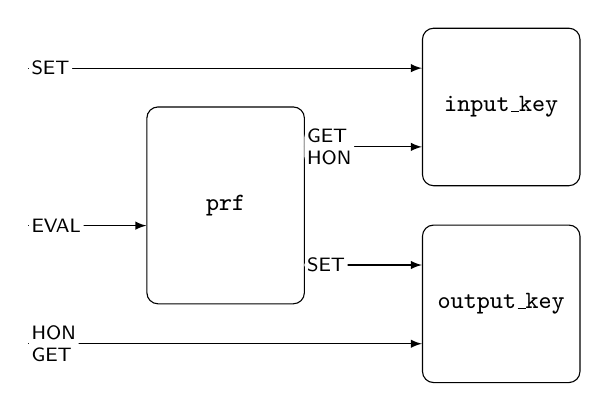
\begin{tikzpicture}
\node[anchor=south west,align=center,package,minimum height=2cm,fill=white] (node0) at (7,3) {\M{input\_key}};\node[anchor=south west,align=center,package,minimum height=2.5cm,fill=white] (node1) at (3.5,1.5) {\M{prf}};\node[anchor=south west,align=center,package,minimum height=2cm,fill=white] (node2) at (7,0.5) {\M{output\_key}};\draw[-latex,rounded corners]
    (5.5,3.5) -- node[onarrow] {\O{GET}\\\O{HON}} (7,3.5);
\draw[-latex,rounded corners]
    (5.5,2) -- node[onarrow] {\O{SET}} (7,2);
\draw[-latex,rounded corners] (2,4.5) -- node[onarrow] {\O{SET}} (7,4.5);
\draw[-latex,rounded corners] (2,2.5) -- node[onarrow] {\O{EVAL}} (3.5,2.5);
\draw[-latex,rounded corners] (2,1) -- node[onarrow] {\O{HON}\\\O{GET}} (7,1);
\end{tikzpicture}

 \caption{Packages of the Unique PRF game.}
\end{figure}

\begin{definition}[PRF]
\label{advantage:assumption:PRF:PRF_mon_real:PRF_mon_ideal}
For all adversaries $\adv$, we define the PRF advantage as\[\mathsf{Adv}(\adv;PRF\_mon\_real,PRF\_mon\_ideal):=\abs{\begin{array}{l}\phantom{-}\prob{1 = \adv\rightarrow PRF\_mon\_real}\\-\prob{1 = \adv\rightarrow PRF\_mon\_ideal}\end{array}},
                      \]where PRF\_mon\_real and PRF\_mon\_ideal are defined in Sec.~\ref{section:game:PRF_mon_real} and Sec.~\ref{section:game:PRF_mon_ideal}, respectively.\end{definition}
\begin{definition}[CR]
\label{advantage:assumption:CR:CR_real:CR_ideal}
For all adversaries $\adv$, we define the CR advantage as\[\mathsf{Adv}(\adv;CR\_real,CR\_ideal):=\abs{\begin{array}{l}\phantom{-}\prob{1 = \adv\rightarrow CR\_real}\\-\prob{1 = \adv\rightarrow CR\_ideal}\end{array}},
                      \]where CR\_real and CR\_ideal are defined in Sec.~\ref{section:game:CR_real} and Sec.~\ref{section:game:CR_ideal}, respectively.\end{definition}

\begin{definition}[Unique PRF]
\label{advantage:theorem:Main:PRF_real:PRF_ideal}
For all adversaries $\adv$, we define the Main advantage as\[\mathsf{Adv}(\adv;PRF\_real,PRF\_ideal):=\abs{\begin{array}{l}\phantom{-}\prob{1 = \adv\rightarrow PRF\_real}\\-\prob{1 = \adv\rightarrow PRF\_ideal }\end{array}},
                      \]where PRF\_real and PRF\_ideal are defined in Sec.~\ref{section:game:PRF_real} and Sec.~\ref{section:game:PRF_ideal}, respectively.\end{definition}






\section{KEM-HKDF}
\label{section:kem-hkdf}
In this chapter, we will construct KEM-HKDF, a key-binding KEM, from a KEM and the Unique PRF we constructed in the previous section.

\begin{figure}
 \centering
 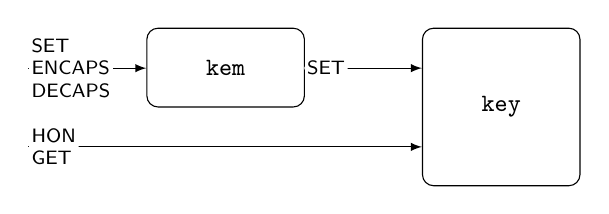
\begin{tikzpicture}
\node[anchor=south west,align=center,package,minimum height=1cm,fill=white] (node0) at (3.5,1.5) {\M{kem}};\node[anchor=south west,align=center,package,minimum height=2cm,fill=white] (node1) at (7,0.5) {\M{key}};\draw[-latex,rounded corners]
    (5.5,2) -- node[onarrow] {\O{SET}} (7,2);
\draw[-latex,rounded corners] (2,2) -- node[onarrow] {\O{SET}\\\O{ENCAPS}\\\O{DECAPS}} (3.5,2);
\draw[-latex,rounded corners] (2,1) -- node[onarrow] {\O{HON}\\\O{GET}} (7,1);
\end{tikzpicture}

 \caption{KEM-HKDF}
 \label{fig:graph_KEM-HKDF}
\end{figure}

The KEM provides three interfaces: SET, ENCAPS, and DECAPS (see also Figure~\ref{fig:Pkg_KEM-HKDF}). SET takes as input a secret key and a n honesty value. If the key is supposed to be honest, we sample a random key and return the corresponding public key. If the key is supposed to be dishonest, we compute the public key based on the secret key provided by the adversary. Both the secret key and the honesty value are saved under the public key.

ENCAPS takes a public key, a randomness, and an honesty value for the randomness as input. If the randomness is supposed to be honest, it is resampled, otherwise, we uses the randomness provided by the adversary. We then in a first step compute the encapsulation, and use the resulting key to compute the PRF of the public key and the ciphertext. We save the combination of public key, ciphertext, and the derived key in the Key package, and set the corresponding honesty bit if both the randomness as well as the key were honest.

DECAPS, on input public key and ciphertext, retrieves the corresponding secret key, and uses this to compute the decapsulation and the derived key. Finally, we set the honesty bit for this public key and ciphertext pair to false.

\begin{figure}
 \centering
 \begin{pcvstack}\underline{\underline{\M{KEM-HKDF}}}\\\begin{pchstack}
\procedure{$\O{SET}(\n{sk}, \n{hon})$}{
\pcif \n{hon} \pcthen\\
\pcind \n{sk} \stackrel{sk}{\sample} \bin^{\n{sk}_\n{len}}\\
 \n{pk} \gets \O{\n{keygen}}(\n{sk})\\
\pcassert \n{HON}[\n{pk}] = \O{none}\left(\O{Type { kind: Boolean }}\right) \\
 \n{SK}\left[\n{pk}\right] \gets \O{some}\left(\n{sk}\right)\\
 \n{HON}\left[\n{pk}\right] \gets \O{some}\left(\n{hon}\right)\\
 \pcreturn \n{pk}\\
}
\pchspace
\procedure{$\O{ENCAPS}(\n{pk}, \n{rand}, \n{hon\_rand})$}{
\pcif \n{hon}_\n{rand} \pcthen\\
\pcind \n{rand} \stackrel{rand}{\sample} \bin^{\n{rand}_\n{len}}\\
 \n{hon}_\n{pk} \gets \O{unwrap}\left(\n{HON}[\n{pk}]\right)\\
 \left(\n{ctxt}, \n{ss}\right) \gets \O{\n{encaps}}(\n{pk}, \n{rand})\\
 \n{hon} \gets \left(\n{hon}_\n{rand} \wedge \n{hon}_\n{pk}\right)\\
 \n{k} \gets \O{\n{prf}}(\n{ss}, \left(\begin{array}{c}\n{pk}, \n{ctxt}\end{array}\right))\\
\O{SET}(\left(\begin{array}{c}\n{pk}, \n{ctxt}\end{array}\right), \n{k}, \n{hon}) \pccomment{Pkg: key} \\
 \pcreturn \n{ctxt}\\
}
\pchspace
\end{pchstack}
\pcvspace
\procedure{$\O{DECAPS}(\n{pk}, \n{ctxt})$}{
 \n{sk} \gets \O{unwrap}\left(\n{SK}[\n{pk}]\right)\\
 \n{ss} \gets \O{\n{decaps}}(\n{sk}, \n{ctxt})\\
 \n{k} \gets \O{\n{prf}}(\n{ss}, \left(\begin{array}{c}\n{pk}, \n{ctxt}\end{array}\right))\\
\O{SET}(\left(\begin{array}{c}\n{pk}, \n{ctxt}\end{array}\right), \n{k}, \lit{false}) \pccomment{Pkg: key} \\
}
\pcvspace\end{pcvstack}

 \caption{KEM}
 \label{fig:Pkg_KEM-HKDF}
\end{figure}

To define security, we again define two worlds, KEM-HKDF\_Real and KEM-HKDF\_Ideal, where the real world works as described above, and for the ideal world, we configure the Key package such that it will always sample random keys instead of the ones provided by KEM-HKDF, and ensure that the resulting keys are unique.

\begin{definition}[KEM-HKDF]
\label{advantage:theorem:Main:Real:Ideal}
For all adversaries $\adv$, we define the KEM-HKDF advantage as\[\mathsf{Adv}(\adv;KEM-HKDF\_Real,KEM-HKDF\_Ideal):=\abs{\begin{array}{l}\phantom{-}\prob{1 = \adv\rightarrow KEM-HKDF\_Real}\\-\prob{1 = \adv\rightarrow KEM-HKDF\_Ideal }\end{array}}.
\]
We say that the KEM-HKDF is secure if this advantage is negligible.
\end{definition}

We need two assumptions to prove KEM-HKDF security: The first one is the Unique PRF security from the previous section (see Definition~\ref{advantage:theorem:Main:PRF_real:PRF_ideal}, and the second one is the security of the underlying KEM. The KEM works similar to the KEM-HKDF, just without the PRF step (see Figure~\ref{fig:Pkg_KEM}).

\begin{figure}
 \centering
 \begin{pcvstack}\underline{\underline{\M{kem}}}\\\begin{pcvstack}
\input{content/domino_imports/Oracle_kem_SET_in_Game_CCA_KEM_Mod.tex}\pcvspace
\procedure{$\O{ENCAPS}(\n{pk}, \n{rand}, \n{hon\_rand})$}{
\pcif \n{hon}_\n{rand} \pcthen\\
\pcind \n{rand} \stackrel{rand}{\sample} \bin^{\n{rand}_\n{len}}\\
 \left(\n{ctxt}, \n{ss}\right) \gets \O{\n{encaps}}(\n{pk}, \n{rand})\\
 \n{hon}_\n{pk} \gets \O{unwrap}\left(\n{HON}[\n{pk}]\right)\\
 \n{hon} \gets \left(\n{hon}_\n{rand} \wedge \n{hon}_\n{pk}\right)\\
\O{SET}(\left(\begin{array}{c}\n{pk}, \n{ctxt}\end{array}\right), \n{ss}, \n{hon}) \pccomment{Pkg: key} \\
 \pcreturn \n{ctxt}\\
}
\pcvspace
\procedure{$\O{DECAPS}(\n{pk}, \n{ctxt})$}{
 \n{sk} \gets \O{unwrap}\left(\n{SK}[\n{pk}]\right)\\
 \n{ss} \gets \O{\n{decaps}}(\n{sk}, \n{ctxt})\\
\O{SET}(\left(\begin{array}{c}\n{pk}, \n{ctxt}\end{array}\right), \n{ss}, \lit{false}) \pccomment{Pkg: key} \\
}
\pcvspace
\end{pcvstack}\end{pcvstack}

 \caption{KEM}
 \label{fig:Pkg_KEM}
\end{figure}

We define the KEM in the real world as above, while in the ideal world, we configure the Key package to always sample random keys instead of the ones provided by the KEM. Note that we do not require uniqueness here. This now let's us define security of a KEM as follows:


\begin{definition}[KEM]
\label{advantage:assumption:KEM:KEM_Mod_real:KEM_Mod_ideal}
For all adversaries $\adv$, we define the KEM advantage as\[\mathsf{Adv}(\adv;KEM\_Mod\_real,KEM\_Mod\_ideal):=\abs{\begin{array}{l}\phantom{-}\prob{1 = \adv\rightarrow KEM\_Mod\_real}\\-\prob{1 = \adv\rightarrow KEM\_Mod\_ideal}\end{array}}.
\]
A KEM is secure if the above advantage is negligible for all adversaries.
\end{definition}

This now lets us state our main theorem for this section:

\begin{theorem}[Main]
We prove that for all adversaries $\adv$, there are reductions $\rdv_{1}$, $\rdv_{2}$ such that \begin{align*}\mathsf{Adv}(\adv, Real, Ideal)) \leq &\mathsf{Adv}(\adv\rightarrow\rdv_{1},\mathit{KEM\_Mod\_ideal},\mathit{KEM\_Mod\_real}) \\+ &\mathsf{Adv}(\adv\rightarrow\rdv_{2},\mathit{Unique\_PRF\_ideal},\mathit{Unique\_PRF\_real}).\end{align*} %where reduction $\rdv_1$ is defined in Fig.~\ref{figure:reduction:KEM:Hybrid0:Hybrid1}, reduction $\rdv_2$ is defined in Fig.~\ref{figure:reduction:Unique_PRF:Hybrid1:Hybrid2}
\end{theorem}







\bibliography{cryptobib/abbrev3,cryptobib/crypto,local}{}
\bibliographystyle{abbrv}

\end{document}
